\begin{frame}
    \begin{center}
        \Huge Neural Networks \\ An introduction
    \end{center}
\end{frame}

\begin{frame}{Neural Networks - Processing information}
\begin{tabular}{p{5cm}|p{5cm}}
    \begin{figure}
    	
\includegraphics[scale = 0.09]{brain}
    \end{figure}
    & 
    \begin{figure}
    	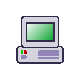
\includegraphics[scale = 1.4]{machine}
    \end{figure} \\
  \multicolumn{1}{c|}{Humam senses} & \multicolumn{1}{c}{Input variables} \\
    \begin{itemize}
        \item Extraction of relevant info
        \item Impossible for machines
    \end{itemize}
    & 
    \begin{itemize}
      \item Preprocessed by user
      \item {e.g.} kinematic variables
    \end{itemize} \\
\multicolumn{1}{c|}{Human brain} & \multicolumn{1}{c}{Net of nodes} \\
    \begin{itemize}
        \item Web of neuron cells
        \item Input from surrounding cells
        \item Single combination $\rightarrow$ action
    \end{itemize}
    & 
    \begin{itemize}
      \item Nodes = simple processors
      \item Connected by linear function
      \item Combination forms non-linear model
    \end{itemize} 
 \end{tabular}
\end{frame}


\begin{frame}{Neural network structure}
\begin{figure}
\centering
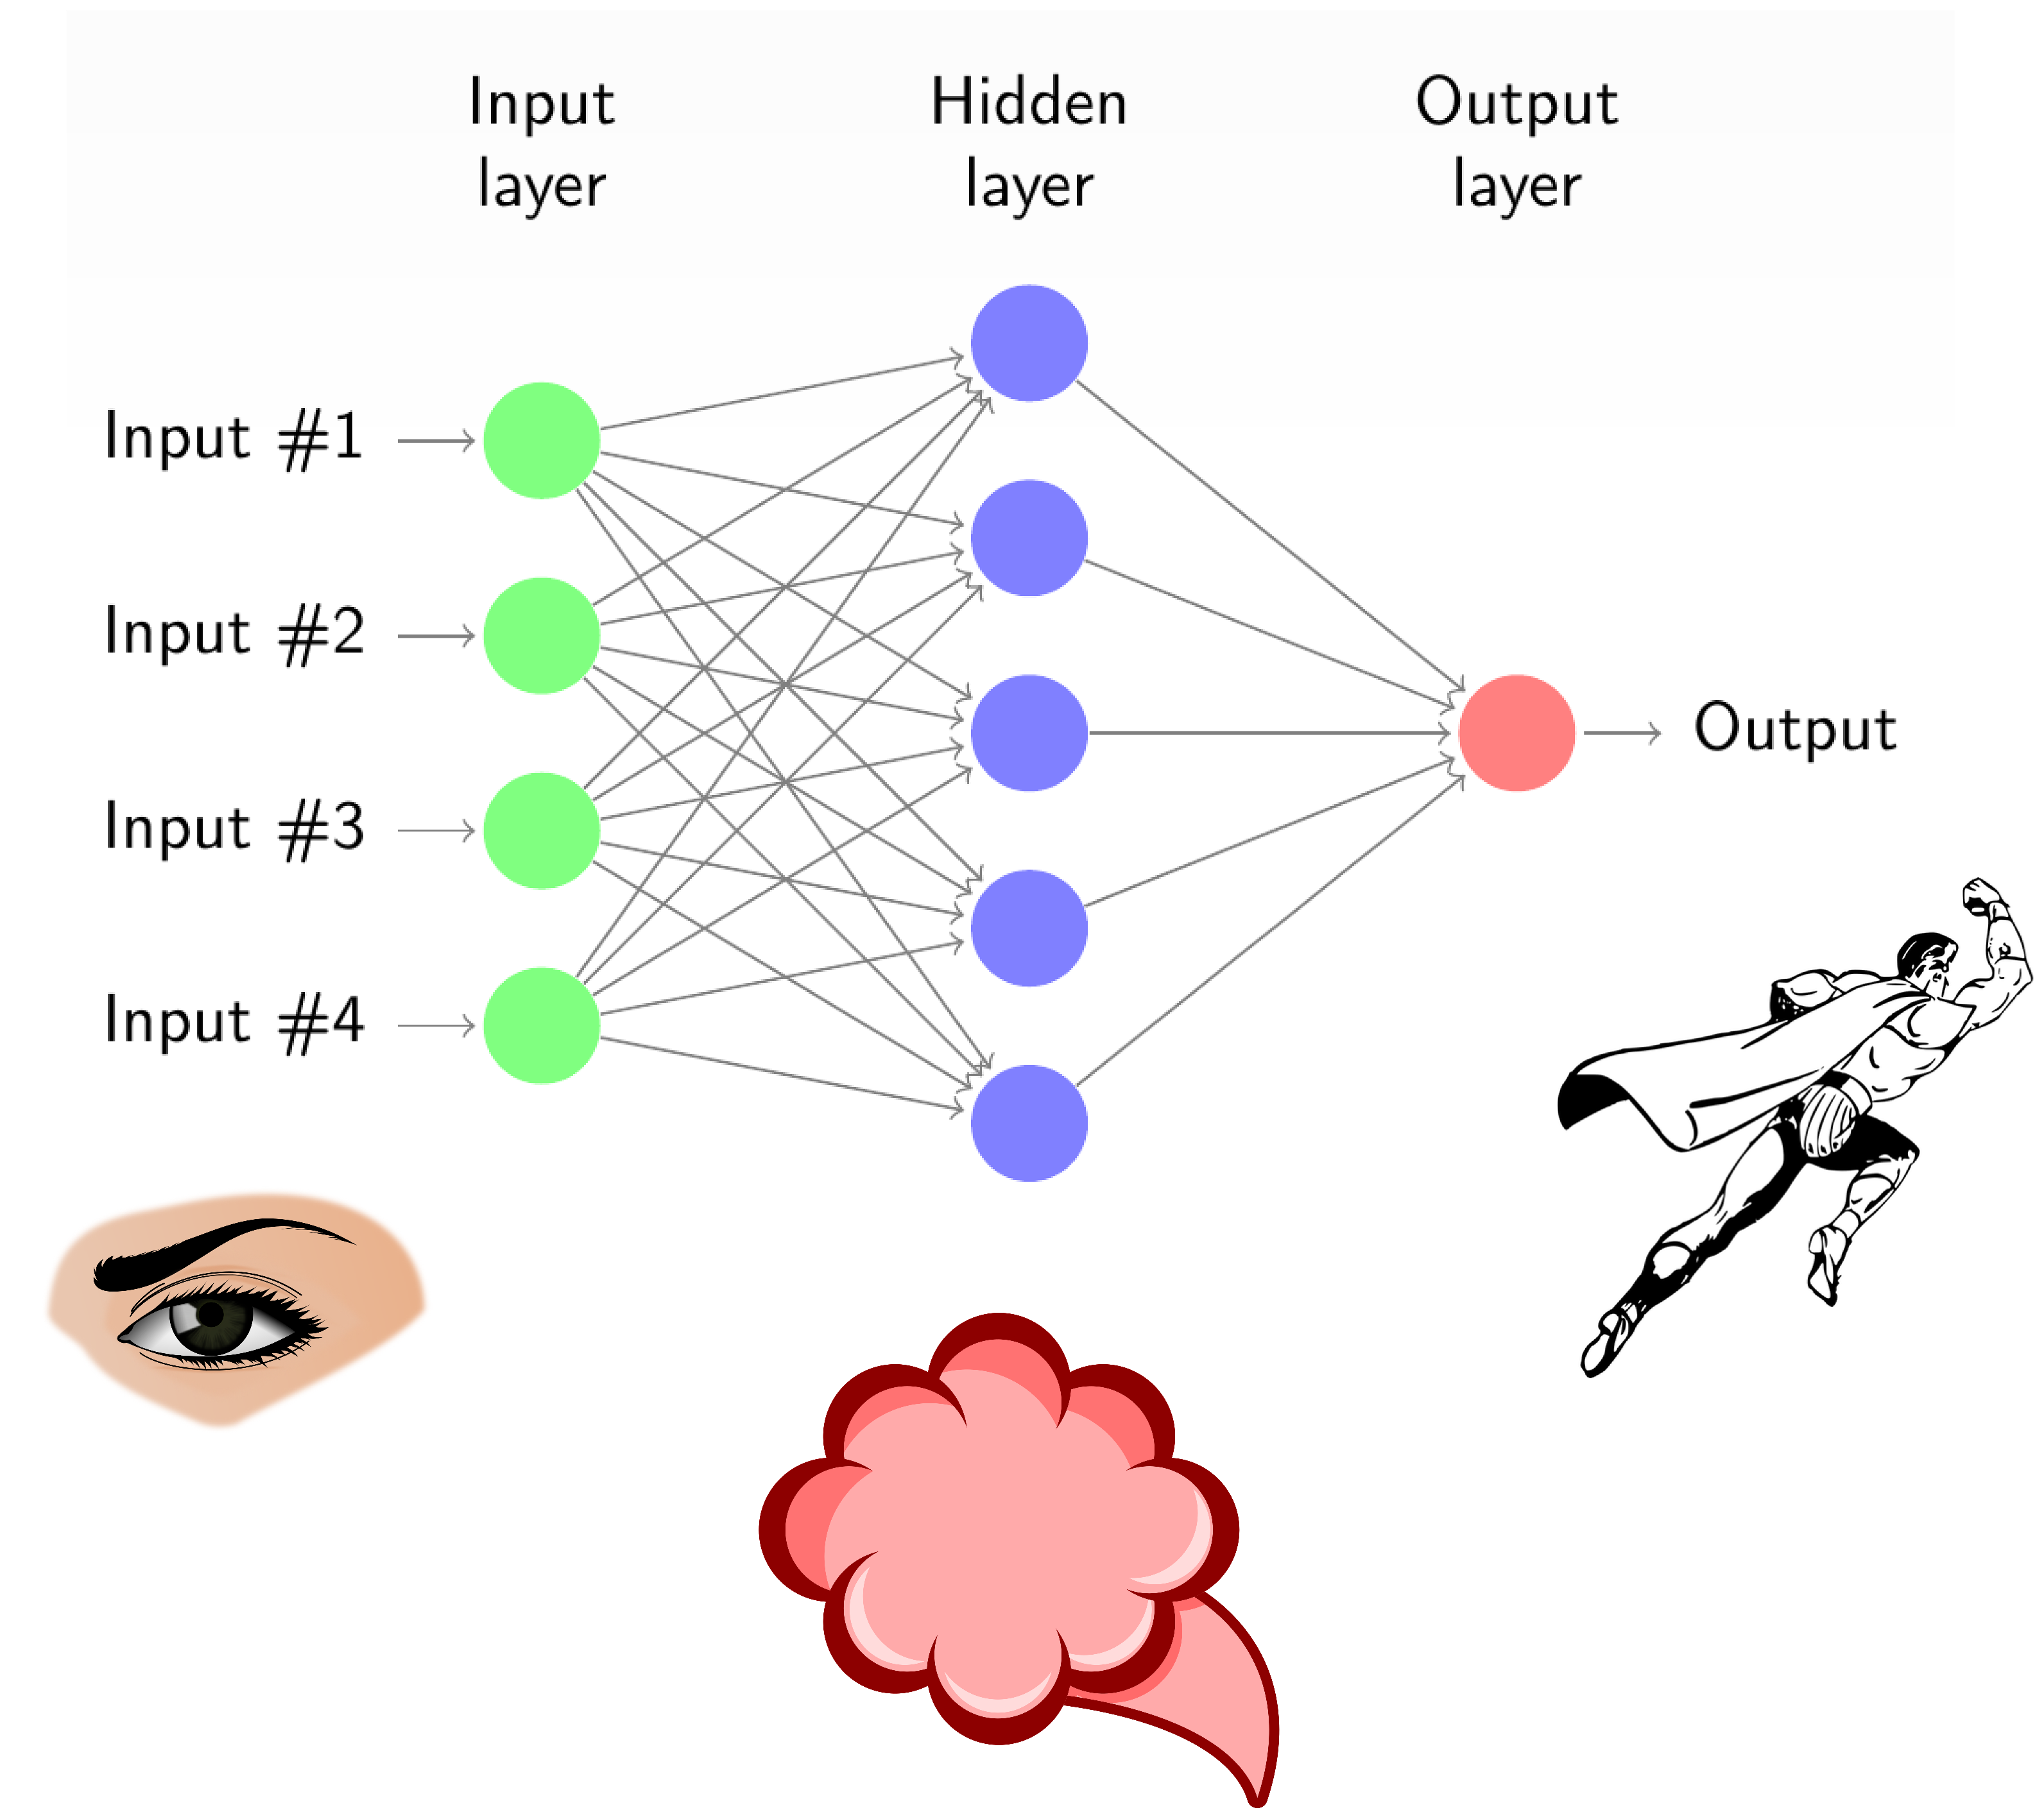
\includegraphics[width=0.8\textwidth]{net_structure}
\end{figure}
\end{frame}

\begin{frame}{Neural Networks - Choosing the next step}
\begin{tabular}{p{5cm}|p{5cm}}
    \begin{figure}
    	
\includegraphics[scale = 0.09]{brain}
    \end{figure}
    & 
    \begin{figure}
    	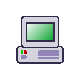
\includegraphics[scale = 1.4]{machine}
    \end{figure} \\
  \multicolumn{1}{c|}{Evaluation of an action} & \multicolumn{1}{c}{Loss function} \\
    \begin{itemize}
        \item Simple perceptions: pain, satisfaction
        \item Expectation
    \end{itemize}
    & 
    \begin{itemize}
      \item Supervised learning: compare to the desired outcome
      \item Loss = estimator for quality
    \end{itemize} \\
\multicolumn{1}{c|}{Decision for a next step} & \multicolumn{1}{c}{Optimisation} \\
    \begin{itemize}
        \item Trial and error
        \item Learning from experience
    \end{itemize}
    & 
    \begin{itemize}
      \item Back-propagation impact of parameters' on the loss
      \item Adjust parameters to minimise plot
    \end{itemize} 
 \end{tabular}
\end{frame}

\begin{frame}{Hyperparameter optimisation}
    \begin{block}{What is a hyperparameter?}
        \begin{itemize}
            \item During the learning process the neural network optimises its internal parameters
            \item Some parameters are still set by the user according to the task of the network
            \item These are called hyperparameters
        \end{itemize}
        
    \end{block}
    \begin{block}{How does one optimise the choice?}
        \begin{itemize}
            \item Neural networks provide several metrics to estimate result and performance
            \item To optimise the hyperparameters one usually runs several configurations to find a good set of parameters
        \end{itemize}
    \end{block}
\end{frame}


\begin{frame}{Hyperparameters to remember}
    \begin{block}{The core}
        \begin{enumerate}
            \item[Nodes] number of computational units
            \item[Layers] depth of computational units
            \item[Epochs] duration of training
            \item[Batchsize] batch of data we look at per time
        \end{enumerate}
    \end{block}
    \begin{block}{Stuff you will encounter}
        \begin{enumerate}
            \item[Dropout] regularises, creates flexibility
            \item[Optimiser] calculates the next step
            \item[Activation function] creates non-linearity
    \end{enumerate}
    \end{block}
\end{frame}